CSP Anlagen beziehen ihre prim�re Energiequelle aus der Direct Normal Irradiance (DNI), welche im besten Fall in einem rechten Winkel zu einer Oberfl�che ausgerichtet ist, die in der Lage ist die Sonnenstrahlung aufzunehmen. Dieses Potential ist im sogenannten �sun belt� am gr��ten. Der �sun belt� bezeichnet den Bereich der Erde n�rdlich und s�dlich vom zwanzigsten bis zum vierzigsten Breitengrad. Zum jetzigen Zeitpunkt wurden vier Haupttechnologien entwickelt und getestet:

\begin{itemize}
	\item Parabolrinnenkraftwerke
	\item Fresnelrinnenkraftwerke
	\item Solarturmkraftwerke
\end{itemize}

\begin{figure}[H]
	\centering
	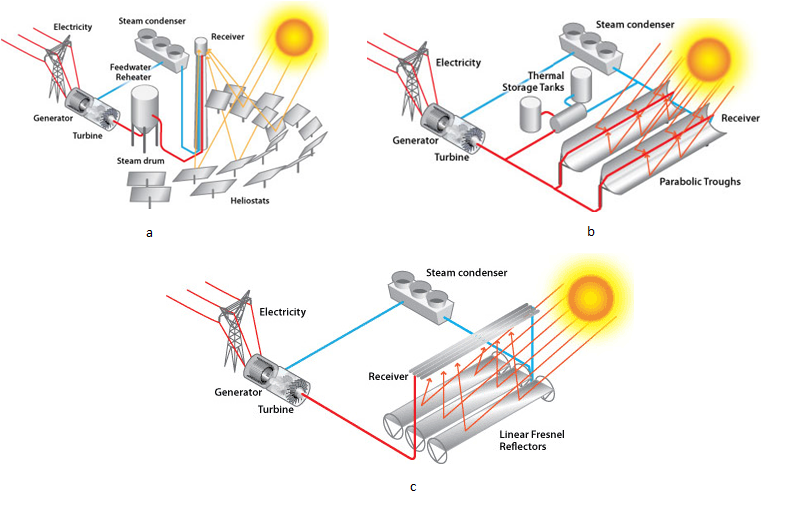
\includegraphics[width=0.9\textwidth]{technik.png}
	\caption{CSP Technologien}
	\label{fig:technik}
\end{figure}

\textbf{Parabolrinnenkraftwerke}
\newline
Ein Parabolrinnenkraftwerk besteht aus einer Reihe von parabelf�rmigen Sonnenkollektoren und einer Gasturbine zur Erzeugung von elektrischer Energie. Zur �berf�hrung der W�rmeenergie von den Kollektoren zur Turbine wird eine Transferfl�ssigkeit verwendet. Diese besteht meistens aus einem synthetisch hergestellten �l, welches durch die Kollektoren flie�t. Das �l wird im Anschluss zur Erzeugung von hei�em Dampf genutzt, was schlussendlich durch die Turbine str�mt. F�r die Zukunft werden neue Technologien im Bereich der Transferfl�ssigkeit angestrebt. So sind L�sungen ohne den Gebrauch von �l erstrebenswert, da die Verwendung von �l mit hohen Kosten in der Aufbereitung und Entsorgung verbunden ist. Auch ist die Verwendung von geschmolzenem Sand in der Entwicklung, welches gegen�ber �l eine h�here Effizienz erzielt, da weitaus h�here Temperaturen erreicht werden k�nnen.

\textbf{Fresnelrinnenkraftwerke} 
\newline
Im Gegensatz zu Parabolrinnenkraftwerke setzen Fresnelrinnenkraftwerke auf ebene Kollektoren, die im Gegensatz zur Parabolkollektoren die Sonnenstrahlung auf nur einer Achse aufnehmen. Dies hat eine Effizienzminderung zu Folge, da nicht alle Bereiche des Kollektors orthogonal zur Strahlenrichtung ausgerichtet sind. Die Idee der Fresnel Technologie besteht darin, dass durch die Vereinfachte Technik und die dadurch geringeren Kosten den Verlust der Energie kompensieren.

\textbf{Solarturmkraftwerke}
\newline
Solarturmkraftwerke bestehen aus einem Feld von  Kollektoren, die leicht geneigt die Sonnenstrahlung auf einen in der Mitte des Feldes befindlichen Turm reflektieren. Im Turm werden die geb�ndelten Strahlen dazu genutzt um wieder eine Transferfl�ssigkeit zu erhitzen, welche zur Erzeugung von Dampf genutzt wird. Ein Vorteil bei diesem Ansatz gegen�ber oben Genannten, ist der geringe Transportweg der Energie bis zu Erzeugung von elektrischer Energie. Die Turbine befindet sich meistens direkt im Turm selbst, sodass keine langen Transportwege n�tig sind.
\newline

\begin{figure}[H]
	\centering
	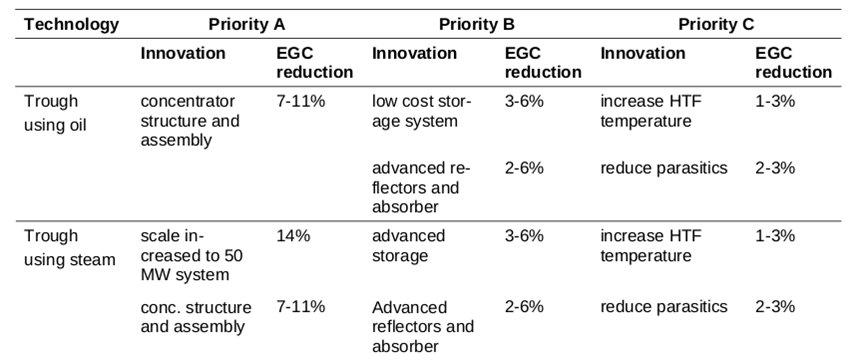
\includegraphics[width=0.9\textwidth]{technische_entwicklung1.png}
	\caption{Technische Entwicklung}
	\label{fig:technik_e1}
\end{figure}

Allgemein sind technische Entwicklungen f�r die Zukunft vor allem in den Bereichen Reflektoren, Speicher, Skalierbarkeit und Temperatur anzusehen (vgl. abb.).
\newline
Reflektoren k�nnen in Bezug auf Widerstandsf�higkeit, Reflektionsgrad, Wirkungsgrad, Gewicht und Zusammenbau weiter optimiert werden. Desweitern besteht Innovationspotential f�r neue Transferfl�ssigkeiten, die zum Transport der W�rme n�tig sind.

\begin{figure}[H]
	\centering
	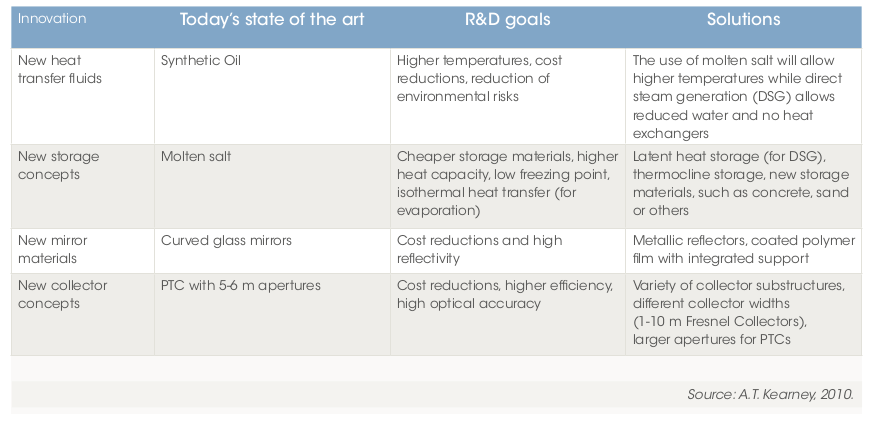
\includegraphics[width=0.9\textwidth]{technische_entwicklung2.png}
	\caption{Technische Entwicklung}
	\label{fig:technik_e2}
\end{figure}

\newline
Um die gewonnene Energie zwischen zu speichern sind moderne Speichertechniken gefragt. Hier gibt es ebenfalls neue Konzepte, die mit geschmolzenem Sand arbeiten um eine h�here Hitze Kapazit�t als herk�mmliche Speichermedien zu gew�hrleisten (vgl. abb.)


